
\chapter{Correlation, Association, and the Yule--Simpson Paradox}
 \label{chapter::correlationassociation}
 
 
Causality is central to human knowledge. Two famous quotes from ancient Greeks are below. 


\begin{quote}
``I would rather discover one causal law than be King of Persia.''

---  Democritus 
\end{quote}


\begin{quote}
``We do not have knowledge of a thing until we grasped its cause.''

--- Aristotle 
\end{quote}
 
 
However, the major part of classic statistics is about association rather than causation.  This chapter will review some basic association measures and point out their fundamental limitations. 
 

\section{Traditional view of statistics}

A traditional view of statistics is to infer correlation or association among variables. Based on this view, there is no role for causal inference in statistics. Two famous aphorisms associated with this view are as follows:

\begin{itemize}
\item
``Correlation does not imply causation.''

\item
``You can not prove causality with statistics.'' 
\end{itemize}

This book has a very different view: statistics is crucial for understanding causality. The main focus of this book is to introduce the formal language for causal inference and develop statistical methods to estimate causal effects in randomized experiments and observational studies. 




 
\section{Some commonly-used measures of association}


\subsection{Correlation and regression}
\label{section:correlatioandregressionintro}

The Pearson correlation coefficient between two random variables $Z$ and $Y$ is
$$
\rho_{ZY} = \frac{  \cov(Z, Y)   }{   \sqrt{   \var(Z) \var(Y)   }   } ,
$$
which measures the linear dependence of $Z$ and $Y.$
 

The linear regression of $Y$ on $Z$ is the model 
\begin{equation}
Y = \alpha + \beta Z + \varepsilon ,
\label{eq::short-regression}
\end{equation} 
 where $E(   \varepsilon  ) = 0$ and $E(   \varepsilon  Z ) = 0 $. We can show that the regression coefficient $\beta$ equals  
 $$
 \beta = \frac{  \cov(Z, Y)   }{   \var(Z)    }  = \rho_{ZY}   \sqrt{     \frac{  \var(Y)     }{ \var(Z)  }    }  . 
 %\propto \rho_{XY}  .
 $$
 So $\beta$ and $\rho_{ZY} $ always have the same sign. 
 
 
We can also define multiple regression of $Y$ on $Z$ and $X$: 
\begin{equation}
 Y = \alpha  + \beta Z + \gamma  X + \varepsilon ,
 \label{eq::long-regression}
\end{equation}
 where $E( \varepsilon) = 0, E( \varepsilon Z) = 0$ and $ E( \varepsilon X) = 0$. 
We usually interpret $\beta$ as the ``effect'' of $Z$ on $Y$, {\it holding $X$ constant} or {\it conditioning on $X$} or {\it controlling for $X$}. Chapter \ref{appendix::basic-linear-regression} reviews the basics of linear regression. 

 

More interestingly, the $\beta$'s in the above two regressions \eqref{eq::short-regression} and \eqref{eq::long-regression} can be different; they can even have different signs. The following \ri{R} code reanalyzed the LaLonde observational data used by \citet{hainmueller2012entropy}. The main question of interest is the ``causal effect'' of a job training program on earnings. The regression controlling for all covariates gives a  coefficient \ri{1067.5461} for \ri{treat}, whereas the regression not controlling for any covariates gives a coefficient \ri{-8506.4954} for \ri{treat}. 


\begin{lstlisting}
> dat <- read.table("cps1re74.csv", header = TRUE)
> dat$u74 <- as.numeric(dat$re74==0)
> dat$u75 <- as.numeric(dat$re75==0)
> 
> ## linear regression on the outcome
> ## . means regression on all other variable in dat
> lmoutcome = lm(re78 ~ ., data = dat)
> round(summary(lmoutcome)$coef[2, ], 3)
  Estimate Std. Error    t value   Pr(>|t|) 
  1067.546    554.060      1.927      0.054 
> 
> lmoutcome = lm(re78 ~ treat, data = dat)
> round(summary(lmoutcome)$coef[2, ], 3)
  Estimate Std. Error    t value   Pr(>|t|) 
 -8506.495    712.766    -11.934      0.000 
\end{lstlisting} 



 
 
 \subsection{Contingency tables}
 \label{sec::twobytwotables-withresume}
 
 We can represent the joint distribution of two binary variables $Z$ and $Y$ by a two-by-two contingency table. With $p_{zy} = \pr( Z=z, Y=y )$, we can summarize the joint distribution in the following table:
 
 
 \begin{center}
\begin{tabular}{lcc}
\hline 
        & $Y =1$ & $Y =0$\\\hline
$Z =1$ & $p_{11}$ & $p_{10}$\\ 
$Z =0$ & $p_{01}$ & $p_{00}$\\ 
\hline 
\end{tabular}
\end{center}
 
 
 Viewing $Z$ as the treatment or exposure and $Y$ as the outcome, we can define the risk difference as
\begin{eqnarray*}
\RD  &=& \pr(Y=1\mid Z=1) - \pr(Y=1\mid Z=0)  \\
&=& \frac{p_{11}}{ p_{11} + p_{10} } -  \frac{p_{01}}{ p_{01} + p_{00} } ,
\end{eqnarray*}
 the risk ratio as
\begin{eqnarray*}
 \RR &=&  \frac{ \pr(Y=1\mid Z=1)  }{    \pr(Y=1\mid Z=0)    }  \\
& =&   \frac{p_{11}}{ p_{11} + p_{10} }  \Big /  \frac{p_{01}}{ p_{01} + p_{00} } ,
\end{eqnarray*}
 and the odds ratio\footnote{In probability theory, the odds of an event is defined as the ratio of the probability that the event happens over the probability that the event does not happen.} as
\begin{eqnarray*}
 \OR &=& \frac{ \pr(Y=1\mid Z=1) /  \pr(Y=0\mid Z=1)  }{    \pr(Y=1\mid Z=0) /\pr(Y=0\mid Z=0)   }  \\
& =& \frac{      \frac{p_{11}}{ p_{11} + p_{10} } /  \frac{p_{10}}{ p_{11} + p_{10} }  }{  \frac{p_{01}}{ p_{01} + p_{00} } / \frac{p_{00}}{ p_{01} + p_{00} }     }  \\
 &=& \frac{ p_{11} p_{00}  }{  p_{10} p_{01} }.
\end{eqnarray*}

The terminology ``risk difference'', ``risk ratio'', and ``odds ratio'' comes from epidemiology. Because the outcomes in epidemiology are often diseases, it is natural to use the name ``risk'' for the probability of having diseases. 
 
 
We have the following simple facts about these measures.
\begin{proposition}\label{prop::2x2-independence}
(1) The following statements are all equivalent\footnote{This book uses the notation $\ind$ to denote independence or conditional independence of random variables. The notation is due to \citet{dawid1979conditional}.}: $Z\ind Y $, $\RD = 0$, $\RR = 1$, and $\OR = 1$. 
(2) If $p_{zy}$'s are all positive, then $\RD >0$ is equivalent to $\RR >1$ and is also equivalent to $\OR > 1$. 
(3)
$\OR \approx \RR$ if  $\pr(Y=1\mid Z=1)$ and $ \pr(Y=1\mid Z=0)$ are small. 
\end{proposition}

I leave the proofs of statements (1) and (2) as Problem \ref{hw::2x2-equivalence}. Statement (3) is informal. The approximation holds because the odds $p/(1-p)$ is close to the probability $p$ for rare diseases with $p\approx 0$: by Taylor expansion $p/(1-p) = p + p^2 + \cdots\approx p $. In epidemiology, if the outcome represents the occurrence of a rare disease, then it is reasonable to assume that $\pr(Y=1\mid X=1)$ and $ \pr(Y=1\mid X=0)$ are small. 
 

 
We can also define conditional versions of the \textsc{rd}, \textsc{rr}, and \textsc{or}  if the probabilities are replaced by the conditional probabilities given another variable $X$, i.e., $\pr(Y=1\mid Z=1, X=x) $ and $ \pr(Y=1\mid Z=0, X=x)  .$
 
 
With counts $n_{zy} = \#\{i:  Z_i=z, Y_i=y \}$, we can summarize the observed data in the following two-by-two table:
 \begin{center}
\begin{tabular}{lcc}
\hline 
        & $Y =1$ & $Y =0$\\\hline
$Z =1$ & $n_{11}$ & $n_{10}$\\ 
$Z =0$ & $n_{01}$ & $n_{00}$\\ 
\hline 
\end{tabular}
\end{center}
We can estimate  \textsc{rd}, \textsc{rr}, and \textsc{or}  by replacing the true probabilities by the sample proportions $\hat p_{zy} = n_{zy}  / n$, where $n$ is the total sample size (see Chapter \ref{section::asymptotic-inference-2x2}). In \ri{R}, functions \ri{fisher.test} performs an exact test and \ri{chisq.test} performs an asymptotic test for   $Z \ind Y$ based on a two-by-two table of observed data. 
 
 
 \begin{example}\label{eg::bertrand2004emily-chapter1}
 \citet{bertrand2004emily} conducted a randomized experiment on resumes to study the effect of perceived race on callbacks for interviews. They randomly assigned Black-sounding or White-sounding names on fictitious resumes to help-wanted ads in Boston and Chicago newspapers. The following two-by-two table summarizes perceived race and callback:
 
 \begin{lstlisting} 
> resume = read.csv("resume.csv")
> Alltable = table(resume$race, resume$call)
> Alltable
       
           0    1
  black 2278  157
  white 2200  235
    \end{lstlisting} 


The two rows have the same total count, so it is apparent that White-sounding names received more callbacks. Fisher's exact test below shows that this difference is statistically significant.    
     \begin{lstlisting} 
> fisher.test(Alltable)

	Fisher's Exact Test for Count Data

data:  Alltable
p-value = 4.759e-05
alternative hypothesis: true odds ratio is not equal to 1
95 percent confidence interval:
 1.249828 1.925573
sample estimates:
odds ratio 
  1.549732 
  \end{lstlisting} 
 
 \end{example}
 
\section{An example of the Yule--Simpson Paradox} 

\subsection{Data}
The classic kidney stone example is from \citet{charig1986comparison}, where $Z$ is the treatment with $1$ for an open surgical procedure and $0$ for a small puncture procedure, and $Y$ is the outcome with $1$ for success and $0$ for failure. The treatment and outcome data can be summarized in the following two-by-two table: 

 \begin{center}
\begin{tabular}{lcc}
\hline 
        & $Y =1$ & $Y =0$\\\hline
$Z =1$ & $273$ & $77$\\ 
$Z =0$ & $289$ & $61$\\ 
\hline 
\end{tabular}
\end{center}



The estimated \textsc{rd} is 
$$
\widehat{\RD} = \frac{273}{273 + 77} - \frac{289}{289 + 61} = 78\% - 83\% = -5\% <0. 
$$
Treatment 0 seems better, that is, the small puncture leads to a higher success rate compared to the open surgical procedure. 


However, the data were not from a randomized controlled trial (RCT)\footnote{In an RCT, patients are randomly assigned to the treatment arms. Part \ref{part::rcts} of this book will focus on RCTs.}. Patients receiving treatment $1$ can be very different from patients receiving treatment $0$. A ``lurking variable'' in this study is the severity of the case: some patients have smaller stones and some patients have larger stones. We can split the data according to the size of the stones. 


For patients with smaller stones, the treatment and outcome data can be summarized in the following two-by-two table: 
 \begin{center}
\begin{tabular}{lcc}
\hline 
        & $Y =1$ & $Y =0$\\\hline
$Z =1$ & $81$ & $6$\\ 
$Z =0$ & $234$ & $36$\\
\hline 
\end{tabular}
\end{center}
For patients with larger stones, the treatment and outcome data can be summarized in the following two-by-two  table:  
 \begin{center}
\begin{tabular}{lcc}
\hline 
        & $Y =1$ & $Y =0$\\\hline
$Z =1$ & $192$ & $71$\\ 
$Z =0$ & $55$ & $25$\\
\hline 
\end{tabular}
\end{center}


The latter two tables must add up to the first table:
$$
81 + 192 = 273,\quad 6 + 71 =77,\quad   234 + 55 = 289, \quad 36 + 25 = 61 .  
$$
From the table for patients with smaller stones, the estimated \textsc{rd} is
$$
\widehat{\RD}_\text{smaller} = \frac{81}{81 + 6} - \frac{234}{234 + 36} = 93\% - 87\% = 6\% > 0,
$$
suggesting that treatment 1 is better. From the table for patients with larger stones, the estimated \textsc{rd}  is 
$$
\widehat{\RD}_\text{larger} = \frac{192}{192 + 71} - \frac{55}{55+25} = 73\% - 69\% = 4\% > 0 ,
$$
also suggesting that treatment 1 is better. 


The above data analysis leads to
$$
\widehat{\RD} < 0,\quad
\widehat{\RD}_\text{smaller} >0, \quad
\widehat{\RD}_\text{larger}  > 0 .
$$
Informally, treatment 1 is better for both patients with smaller and larger stones, but treatment 1 is worse for the whole population. This interpretation is quite confusing if the goal is to infer the treatment effect. In statistics, this is called the Yule--Simpson Paradox or Simpson's Paradox in which the marginal association has the opposite sign to the conditional associations at all levels. 




\subsection{Explanation}



Let $X$ be the binary indicator with $X=1$ for smaller stones and $X=0$ for larger stones. 
Let us first take a look at the $X$--$Z$ relationship by comparing the probabilities of receiving treatment 1 among patients with smaller and larger stones:
\begin{eqnarray*}
&& \widehat{\pr}(Z=1 \mid  X=1) - \widehat{\pr}(Z=1 \mid X=0) \\
&=& \frac{81 + 6}{81 + 6 + 234 + 36} - \frac{192+71}{192 + 71 + 55 + 25} \\
&=&  24\% - 77\% \\
&=& - 53\% < 0 .
\end{eqnarray*}
So patients with larger stones tend to take treatment 1 more frequently. Statistically, $X$ and $Z$ have negative association. 


Let us then take a look at the $X$--$Y$ relationship by comparing the probabilities of success among patients with smaller and larger stones: under treatment 1,
\begin{eqnarray*}
&& \widehat{\pr}(Y=1 \mid Z=1,  X=1) - \widehat{\pr}(Y=1 \mid Z=1,  X=0) \\
&=& \frac{81}{81 + 6} - \frac{192}{192 + 71} \\
&=& 93\% - 73\% \\
&=& 20\%
> 0;
\end{eqnarray*}
under treatment 0, 
\begin{eqnarray*}
&& \widehat{\pr}(Y=1 \mid Z=0, X=1) - \widehat{\pr}(Y=1 \mid Z=0,   X=0) \\
&=& \frac{234}{234 + 36} - \frac{55}{55 + 25} \\
&=& 87\% - 69\% \\
&=& 18\% 
> 0.
\end{eqnarray*}
So under both treatment levels, patients with smaller stones have higher success probabilities. Statistically, $X$ and $Y$ have positive association conditional on both treatment levels. 


\begin{figure}
$$
\xymatrix{
 & X\ar_{-}[ld]\ar^{+}[rd] \\ 
Z \ar_{+}[rr] &&Y 
}
$$
\caption{A diagram for the kidney stone example. The signs indicate the associations of two variables, conditioning on other variables pointing to the downstream variable.}\label{fig::kidney-stone}
\end{figure}




We can summarize the qualitative associations in the diagram in Figure \ref{fig::kidney-stone}. In technical terms, the treatment has a positive path $(Z\rightarrow Y)$ and a more negative path $(Z\leftarrow X \rightarrow Y)$ to the outcome, so the overall association is negative between the treatment and outcome. 
In plain English, when less effective treatment 0 is applied more frequently to the less severe cases, it can appear to be a more effective treatment. 




In general, the association between $Z$ and $Y$ can differ qualitatively from the conditional association between $Z$ and $Y$ given $X$ due to the association between $X$ and $Z$ and the association between $X$ and $Y$.  When the Yule--Simpson Paradox happens,  we say that $X$ is a {\it confounding variable} or {\it confounder} for the relationship between $Z$ and $Y$, or $Z$ and $Y$ are {\it confounded} by $X$.  See Chapters \ref{chapter::observational-studies} and \ref{chapter::evalue} for more in-depth discussion. 
 




\subsection{Geometry of the Yule--Simpson Paradox}


Assume that the two-by-two table based on the aggregated data has counts


 \begin{center}
\begin{tabular}{lcc}
\hline 
 whole population       & $Y =1$ & $Y =0$\\\hline
$Z =1$ & $n_{11}$ & $n_{10}$\\ 
$Z =0$ & $n_{01}$ & $n_{00}$\\
\hline 
\end{tabular}
\end{center}


The two two-by-two tables based on subgroups have counts
 \begin{center}
\begin{tabular}{lcc}
\hline 
subpopulation $X=1$        & $Y =1$ & $Y =0$\\\hline
$Z=1$ & $n_{11|1}$ & $n_{10|1}$\\ 
$Z=0$ & $n_{01|1}$ & $n_{00|1}$\\
\hline 
\end{tabular}
\end{center}
for the subgroup with $X=1$ and
 \begin{center}
\begin{tabular}{lcc}
\hline 
subpopulation    $X=0$    & $Y =1$ & $Y =0$\\\hline
$Z =1$ & $n_{11|0}$ & $n_{10|0}$\\ 
$Z =0$ & $n_{01|0}$ & $n_{00|0}$\\
\hline 
\end{tabular}
\end{center}
for the subgroup with $X=0.$


Figure \ref{fig::geomtry-simpson} shows the geometry of the Yule--Simpson Paradox. The y-axis shows the count of successes with $Y=1$ and the x-axis shows the count of failures with $Y=0$. The two parallelograms correspond to aggregating the counts of successes and failures under two treatment levels. The slope of  $OA_1$ is larger than that of $OB_1$, and the slope of  $OA_0$ is larger than that of $OB_0$. So the treatment seems beneficial to the outcome within both levels of $X$. However, the slope of $OA$ is smaller than that of $OB$. So the treatment seems harmful to the outcome for the whole population. The Yule--Simpson Paradox arises. 





\begin{figure}
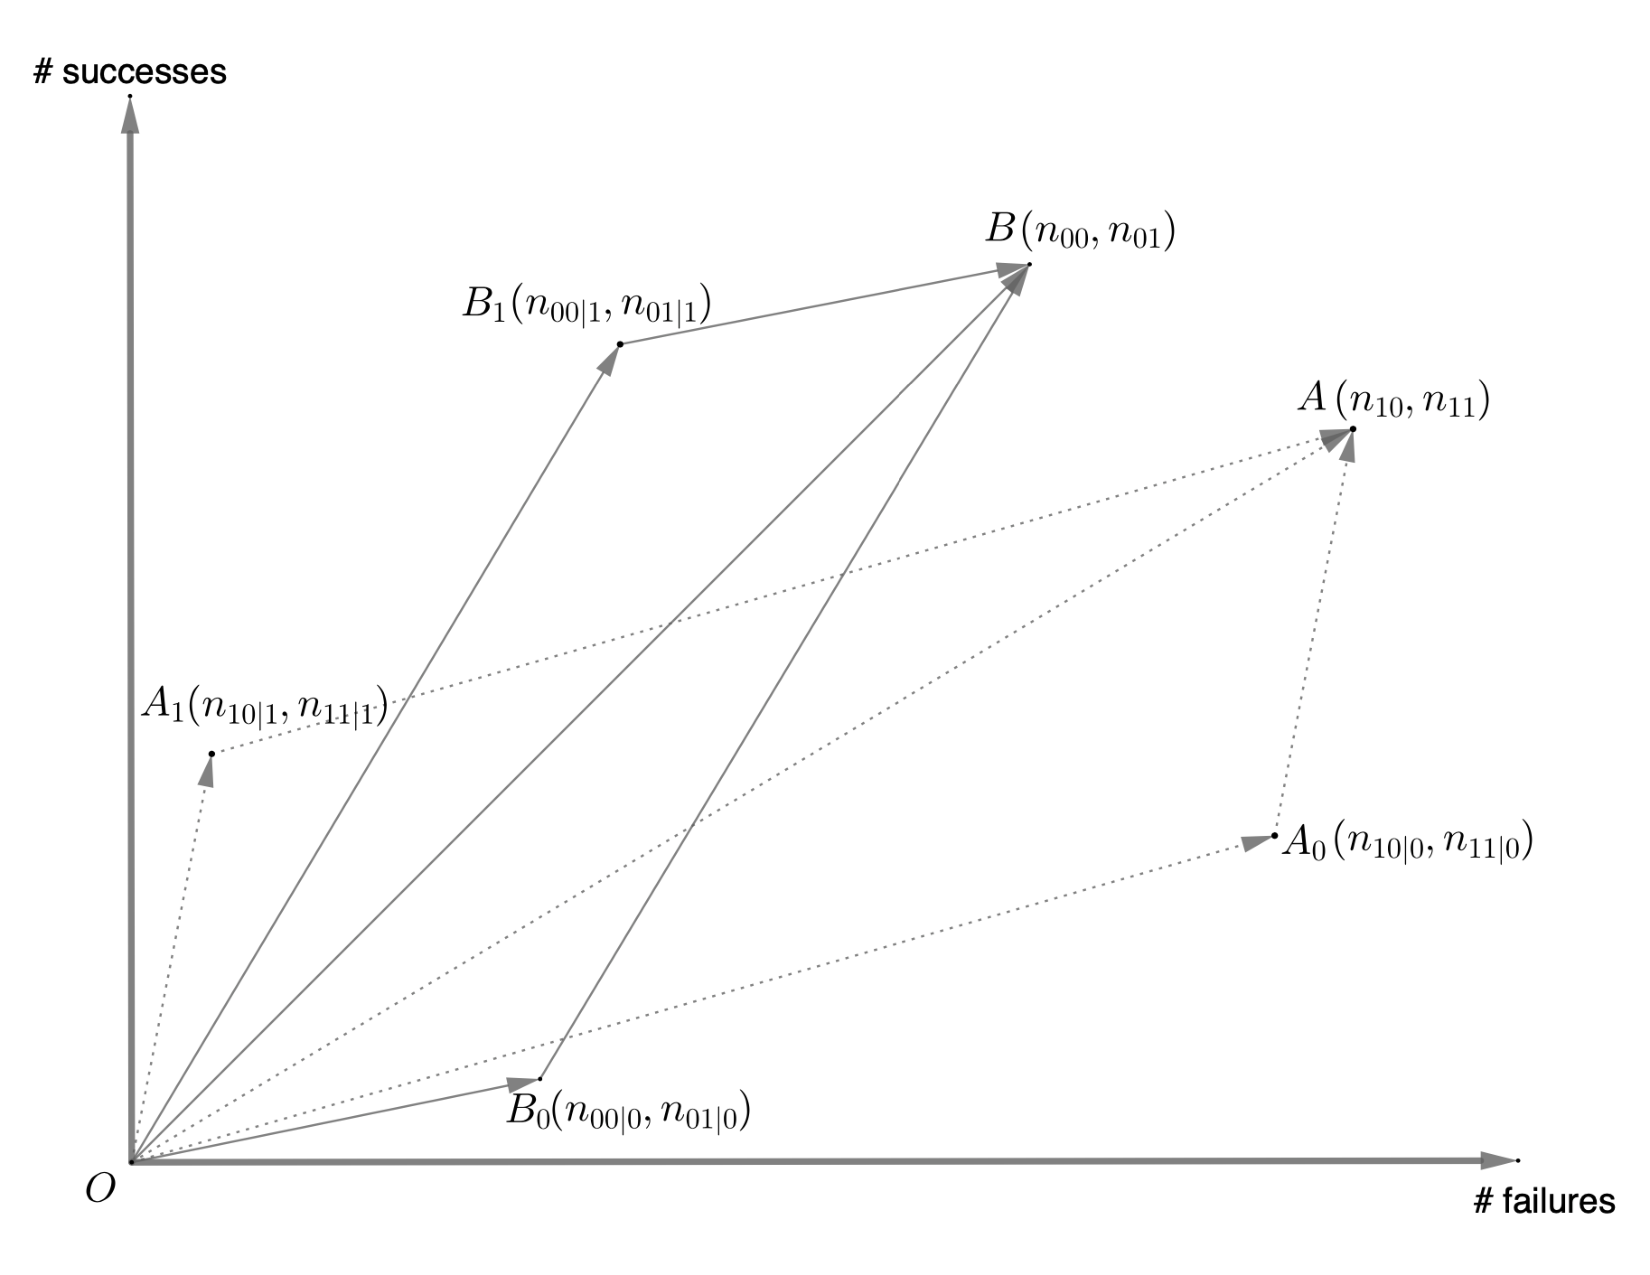
\includegraphics[width=\textwidth]{figures/simpson_geometry2.pdf}
\caption{Geometry of the Yule--Simpson Paradox}\label{fig::geomtry-simpson}
\end{figure}

\section{The Berkeley graduate school admission data}
\label{sec::berkeleydata}

\citet{bickel1975sex} investigated the admission rates of male and female students into the graduate school of Berkeley. The \ri{R} package \ri{datasets} contains the original data \ri{UCBAdmissions}. The raw data by the six largest departments are shown below: 
\begin{lstlisting}
> library(datasets)
> UCBAdmissions = aperm(UCBAdmissions, c(2, 1, 3))
> UCBAdmissions
, , Dept = A

        Admit
Gender   Admitted Rejected
  Male        512      313
  Female       89       19

, , Dept = B

        Admit
Gender   Admitted Rejected
  Male        353      207
  Female       17        8

, , Dept = C

        Admit
Gender   Admitted Rejected
  Male        120      205
  Female      202      391

, , Dept = D

        Admit
Gender   Admitted Rejected
  Male        138      279
  Female      131      244

, , Dept = E

        Admit
Gender   Admitted Rejected
  Male         53      138
  Female       94      299

, , Dept = F

        Admit
Gender   Admitted Rejected
  Male         22      351
  Female       24      317
\end{lstlisting}


Aggregating the data over departments, we have a simple two-by-two table:
\begin{lstlisting} 
> UCBAdmissions.sum = apply(UCBAdmissions, c(1, 2), sum)
> UCBAdmissions.sum
        Admit
Gender   Admitted Rejected
  Male       1198     1493
  Female      557     1278
\end{lstlisting}

The following function, building upon \ri{chisq.test}, have a two-by-two table as the input and the estimated \textsc{rd} and $p$-value as output:
\begin{lstlisting}
> risk.difference = function(tb2)
+ {
+   p1      = tb2[1, 1]/(tb2[1, 1] + tb2[1, 2])
+   p2      = tb2[2, 1]/(tb2[2, 1] + tb2[2, 2])
+   testp   = chisq.test(tb2)
+   
+   return(list(p.diff = p1 - p2,  
+               pv = testp$p.value))	    
+ }
\end{lstlisting}
With this function, we find a large, significant difference between the admission rates of male and female students:
\begin{lstlisting}
> risk.difference(UCBAdmissions.sum)
$p.diff
[1] 0.1416454

$pv
[1] 1.055797e-21
\end{lstlisting}

Stratifying on the departments, we find smaller and insignificant differences between the admission rates of male and female students. In department A, the difference is significant but negative. 
\begin{lstlisting}
> P.diff = rep(0, 6)
> PV     = rep(0, 6)
> for(dd in 1:6)
+ {
+ 	 department = risk.difference(UCBAdmissions[, , dd])
+ 	 P.diff[dd] = department$p.diff
+ 	 PV[dd]     = department$pv 
+ }
> 
> round(P.diff, 2)
[1] -0.20 -0.05  0.03 -0.02  0.04 -0.01
> round(PV, 2)
[1] 0.00 0.77 0.43 0.64 0.37 0.64
\end{lstlisting} 



 



 
\section{Homework Problems}


\paragraph{Independence in two-by-two tables}\label{hw::2x2-equivalence}

Prove (1) and (2) in Proposition \ref{prop::2x2-independence}. 


\paragraph{More examples of the Yule--Simpson Paradox}


Give a numeric example of a two-by-two-by-two table in which the Yule--Simpson Paradox arises. 

Find a real-life example in which the Yule--Simpson Paradox arises. 



\paragraph{Correlation and partial correlation}\label{hw::partial-correlation}

Consider a three-dimensional Normal random vector:
$$
\begin{pmatrix}
X\\
Y\\
Z
\end{pmatrix}
\sim 
\textsc{N}
\left(
\begin{pmatrix}
0\\
0\\
0
\end{pmatrix},
\begin{pmatrix}
1 & \rho_{XY} &\rho_{XZ} \\
  \rho_{XY}  & 1 & \rho_{YZ} \\
  \rho_{XZ} &  \rho_{YZ} & 1
\end{pmatrix}
\right) . 
$$
The correlation coefficient between $Y$ and $Z$ is $\rho_{YZ}$. 
There are many equivalent definitions of the partial correlation coefficient. 
For a multivariate Normal vector, let $\rho_{YZ|X}$ denote the partial correlation coefficient between $Y$ and $Z$ given $X$, which is defined as their correlation coefficient in the conditional distribution $(Y, Z)\mid X$. Show that
$$
\rho_{YZ\mid X} = \frac{   \rho_{YZ} - \rho_{YX} \rho_{ZX}  }{  \sqrt{  1-\rho_{YX}^2 }  \sqrt{1- \rho_{ZX}^2  }  }  . 
$$

Give a numerical example with $\rho_{YZ} > 0$ and $\rho_{YZ|X} < 0$. 

Remark: This is the Yule--Simpson Paradox for a Normal random vector. 
You can use the results in Chapter \ref{sec::multivariate-normal} to prove the formula for the partial correlation coefficient. 



\paragraph{Specification searches}\label{hw::lalonde-obs-reg}

Section \ref{section:correlatioandregressionintro} re-analyzes the data used by \citet{hainmueller2012entropy}. We used the outcome named \ri{re78} and the treatment named \ri{treat} in the analysis. Moreover, the data also contain $10$ covariates and therefore $2^{10} = 1024$ possible subsets of covariates in the linear regression. Run $1024$ linear regressions with all possible subsets of covariates, and report the regression coefficients of the treatment. How many coefficients of the treatment are positively significant, how many are negatively significant, and how many are not significant? You can also report other interesting findings from these regressions.


\paragraph{More on racial discrimination}

Section \ref{sec::twobytwotables-withresume} re-analyzes the data collected by \citet{bertrand2004emily}. Conduct analyses separately for males and females. What do you find from these subgroup analyses?


\paragraph{Recommended reading}

\citet{bickel1975sex} is the original paper for the paradox reported in Section \ref{sec::berkeleydata}. 
\citet{pearl2018book} recently revisited the study from the causal inference perspective. 


